\documentclass[tikz,border=8pt]{standalone}
\usepackage{ctex}
\usepackage{amsmath,amssymb,bm}
\usetikzlibrary{arrows.meta,calc,angles,quotes,patterns,positioning,decorations.pathmorphing}
\definecolor{ink}{RGB}{30,43,58}
\definecolor{blue}{RGB}{37,91,166}
\definecolor{orange}{RGB}{219,113,25}
\definecolor{green}{RGB}{39,139,94}
\definecolor{red}{RGB}{192,52,52}
\tikzset{
  line cap=round,line join=round,
  body/.style={draw=ink,very thick},
  axis/.style={-{Latex[length=2.5mm]},draw=ink,very thick},
  vec/.style={-{Latex[length=2.5mm]},draw=blue,very thick},
  force/.style={-{Latex[length=2.5mm]},draw=red,very thick},
  guide/.style={draw=ink!45,dashed},
  dim/.style={{Latex[length=2mm]}-{Latex[length=2mm]},draw=ink!75}
}

\usetikzlibrary{decorations.pathmorphing}
\tikzset{mass/.style={circle,draw,fill=white,minimum size=7mm},curve/.style={very thick,blue},rope/.style={very thick,blue},ray/.style={very thick,blue,-{Latex}},impulse/.style={very thick,orange,-{Latex}},resistor/.style={thick,decorate,decoration={zigzag,segment length=3mm,amplitude=1mm}}}
\begin{document}
% 1 question-01
\begin{tikzpicture}[x=1cm,y=1cm,font=\small]

\begin{scope}
\coordinate (O) at (0,1.2);\draw[green,very thick] (.8,-.7)--(-.8,3.1) node[above] {$OB$};\draw[orange,very thick] (O)--(1.36,1.774) node[right] {$A$};\draw[body] (1.36,1.774) circle(.6);\draw[guide] (0,1.2)--(0,3.2);\fill (O) circle(2pt) node[left] {$O$};\node[align=center] at (.5,-1.5) {正中位置：$OA\perp OB$\\$OA$ 随主销内倾而倾斜};
\end{scope}
\begin{scope}[xshift=6.7cm]
\draw[body] (-2,0)--(2,0) node[right] {前进方向};\draw[body] (0,1) circle(1);\draw[green,very thick] (.55,0)--(-1.1,3) node[above] {$OB$};\fill (0,0) circle(2pt) node[below] {$P$};\fill (.55,0) circle(2pt) node[below right] {$O'$};\draw[dim] (0,-.7)--(.55,-.7) node[midway,below] {$t$};\node[align=center] at (0,-1.6) {后倾的侧视图\\轴与地面的交点 $O'$ 在 $P$ 前方};
\end{scope}

\end{tikzpicture}

% 2 solution-01
\begin{tikzpicture}[x=1cm,y=1cm,font=\small]

\draw[body] (-2,0)--(2,0);\draw[body] (0,1) circle(1);\draw[green,very thick] (.55,0)--(-1.1,3) node[above] {$OB$};\fill (0,0) circle(2pt) node[below] {$P$};\fill (.55,0) circle(2pt) node[below right] {$O'$};\node[red,above left] at (0,.1) {$\odot F_f$};\draw[dim] (0,-.8)--(.55,-.8) node[midway,below] {$t\simeq r\alpha$};
\node[align=left,anchor=west] at (3.6,1.2) {侧向力垂直纸面，不能画成沿地面的力\\[6pt]主销内倾：$M_1=-Gl\sin\beta\sin\theta/4$\\[6pt]后倾：$F_f\simeq mv^2\theta/(2d)$\\[6pt]$M_2\simeq-F_fr\alpha$};

\end{tikzpicture}

% 3 question-02
\begin{tikzpicture}[x=1cm,y=1cm,font=\small]
\draw[axis] (-3.5,0)--(3.7,0) node[right] {$z$};
\draw[blue,thick] plot coordinates {(-3.000000,-0.900000) (-2.939394,-0.900634) (-2.878788,-0.902534) (-2.818182,-0.905692) (-2.757576,-0.910096) (-2.696970,-0.915728) (-2.636364,-0.922564) (-2.575758,-0.930578) (-2.515152,-0.939737) (-2.454545,-0.950005) (-2.393939,-0.961340) (-2.333333,-0.973696) (-2.272727,-0.987024) (-2.212121,-1.001270) (-2.151515,-1.016376) (-2.090909,-1.032282) (-2.030303,-1.048924) (-1.969697,-1.066235) (-1.909091,-1.084144) (-1.848485,-1.102581) (-1.787879,-1.121470) (-1.727273,-1.140736) (-1.666667,-1.160301) (-1.606061,-1.180086) (-1.545455,-1.200012) (-1.484848,-1.219998) (-1.424242,-1.239964) (-1.363636,-1.259829) (-1.303030,-1.279514) (-1.242424,-1.298939) (-1.181818,-1.318026) (-1.121212,-1.336699) (-1.060606,-1.354881) (-1.000000,-1.372500) (-0.939394,-1.389485) (-0.878788,-1.405767) (-0.818182,-1.421281) (-0.757576,-1.435965) (-0.696970,-1.449758) (-0.636364,-1.462607) (-0.575758,-1.474458) (-0.515152,-1.485265) (-0.454545,-1.494983) (-0.393939,-1.503574) (-0.333333,-1.511003) (-0.272727,-1.517240) (-0.212121,-1.522260) (-0.151515,-1.526043) (-0.090909,-1.528574) (-0.030303,-1.529841) (0.030303,-1.529841) (0.090909,-1.528574) (0.151515,-1.526043) (0.212121,-1.522260) (0.272727,-1.517240) (0.333333,-1.511003) (0.393939,-1.503574) (0.454545,-1.494983) (0.515152,-1.485265) (0.575758,-1.474458) (0.636364,-1.462607) (0.696970,-1.449758) (0.757576,-1.435965) (0.818182,-1.421281) (0.878788,-1.405767) (0.939394,-1.389485) (1.000000,-1.372500) (1.060606,-1.354881) (1.121212,-1.336699) (1.181818,-1.318026) (1.242424,-1.298939) (1.303030,-1.279514) (1.363636,-1.259829) (1.424242,-1.239964) (1.484848,-1.219998) (1.545455,-1.200012) (1.606061,-1.180086) (1.666667,-1.160301) (1.727273,-1.140736) (1.787879,-1.121470) (1.848485,-1.102581) (1.909091,-1.084144) (1.969697,-1.066235) (2.030303,-1.048924) (2.090909,-1.032282) (2.151515,-1.016376) (2.212121,-1.001270) (2.272727,-0.987024) (2.333333,-0.973696) (2.393939,-0.961340) (2.454545,-0.950005) (2.515152,-0.939737) (2.575758,-0.930578) (2.636364,-0.922564) (2.696970,-0.915728) (2.757576,-0.910096) (2.818182,-0.905692) (2.878788,-0.902534) (2.939394,-0.900634) (3.000000,-0.900000)};
\draw[blue,thick] plot coordinates {(-3.000000,-0.600000) (-2.939394,-0.600423) (-2.878788,-0.601689) (-2.818182,-0.603795) (-2.757576,-0.606731) (-2.696970,-0.610485) (-2.636364,-0.615043) (-2.575758,-0.620385) (-2.515152,-0.626492) (-2.454545,-0.633337) (-2.393939,-0.640893) (-2.333333,-0.649131) (-2.272727,-0.658016) (-2.212121,-0.667513) (-2.151515,-0.677584) (-2.090909,-0.688188) (-2.030303,-0.699283) (-1.969697,-0.710823) (-1.909091,-0.722763) (-1.848485,-0.735054) (-1.787879,-0.747647) (-1.727273,-0.760491) (-1.666667,-0.773534) (-1.606061,-0.786724) (-1.545455,-0.800008) (-1.484848,-0.813332) (-1.424242,-0.826642) (-1.363636,-0.839886) (-1.303030,-0.853009) (-1.242424,-0.865960) (-1.181818,-0.878684) (-1.121212,-0.891132) (-1.060606,-0.903254) (-1.000000,-0.915000) (-0.939394,-0.926323) (-0.878788,-0.937178) (-0.818182,-0.947521) (-0.757576,-0.957310) (-0.696970,-0.966506) (-0.636364,-0.975071) (-0.575758,-0.982972) (-0.515152,-0.990177) (-0.454545,-0.996655) (-0.393939,-1.002383) (-0.333333,-1.007335) (-0.272727,-1.011494) (-0.212121,-1.014840) (-0.151515,-1.017362) (-0.090909,-1.019049) (-0.030303,-1.019894) (0.030303,-1.019894) (0.090909,-1.019049) (0.151515,-1.017362) (0.212121,-1.014840) (0.272727,-1.011494) (0.333333,-1.007335) (0.393939,-1.002383) (0.454545,-0.996655) (0.515152,-0.990177) (0.575758,-0.982972) (0.636364,-0.975071) (0.696970,-0.966506) (0.757576,-0.957310) (0.818182,-0.947521) (0.878788,-0.937178) (0.939394,-0.926323) (1.000000,-0.915000) (1.060606,-0.903254) (1.121212,-0.891132) (1.181818,-0.878684) (1.242424,-0.865960) (1.303030,-0.853009) (1.363636,-0.839886) (1.424242,-0.826642) (1.484848,-0.813332) (1.545455,-0.800008) (1.606061,-0.786724) (1.666667,-0.773534) (1.727273,-0.760491) (1.787879,-0.747647) (1.848485,-0.735054) (1.909091,-0.722763) (1.969697,-0.710823) (2.030303,-0.699283) (2.090909,-0.688188) (2.151515,-0.677584) (2.212121,-0.667513) (2.272727,-0.658016) (2.333333,-0.649131) (2.393939,-0.640893) (2.454545,-0.633337) (2.515152,-0.626492) (2.575758,-0.620385) (2.636364,-0.615043) (2.696970,-0.610485) (2.757576,-0.606731) (2.818182,-0.603795) (2.878788,-0.601689) (2.939394,-0.600423) (3.000000,-0.600000)};
\draw[blue,thick] plot coordinates {(-3.000000,-0.300000) (-2.939394,-0.300211) (-2.878788,-0.300845) (-2.818182,-0.301897) (-2.757576,-0.303365) (-2.696970,-0.305243) (-2.636364,-0.307521) (-2.575758,-0.310193) (-2.515152,-0.313246) (-2.454545,-0.316668) (-2.393939,-0.320447) (-2.333333,-0.324565) (-2.272727,-0.329008) (-2.212121,-0.333757) (-2.151515,-0.338792) (-2.090909,-0.344094) (-2.030303,-0.349641) (-1.969697,-0.355412) (-1.909091,-0.361381) (-1.848485,-0.367527) (-1.787879,-0.373823) (-1.727273,-0.380245) (-1.666667,-0.386767) (-1.606061,-0.393362) (-1.545455,-0.400004) (-1.484848,-0.406666) (-1.424242,-0.413321) (-1.363636,-0.419943) (-1.303030,-0.426505) (-1.242424,-0.432980) (-1.181818,-0.439342) (-1.121212,-0.445566) (-1.060606,-0.451627) (-1.000000,-0.457500) (-0.939394,-0.463162) (-0.878788,-0.468589) (-0.818182,-0.473760) (-0.757576,-0.478655) (-0.696970,-0.483253) (-0.636364,-0.487536) (-0.575758,-0.491486) (-0.515152,-0.495088) (-0.454545,-0.498328) (-0.393939,-0.501191) (-0.333333,-0.503668) (-0.272727,-0.505747) (-0.212121,-0.507420) (-0.151515,-0.508681) (-0.090909,-0.509525) (-0.030303,-0.509947) (0.030303,-0.509947) (0.090909,-0.509525) (0.151515,-0.508681) (0.212121,-0.507420) (0.272727,-0.505747) (0.333333,-0.503668) (0.393939,-0.501191) (0.454545,-0.498328) (0.515152,-0.495088) (0.575758,-0.491486) (0.636364,-0.487536) (0.696970,-0.483253) (0.757576,-0.478655) (0.818182,-0.473760) (0.878788,-0.468589) (0.939394,-0.463162) (1.000000,-0.457500) (1.060606,-0.451627) (1.121212,-0.445566) (1.181818,-0.439342) (1.242424,-0.432980) (1.303030,-0.426505) (1.363636,-0.419943) (1.424242,-0.413321) (1.484848,-0.406666) (1.545455,-0.400004) (1.606061,-0.393362) (1.666667,-0.386767) (1.727273,-0.380245) (1.787879,-0.373823) (1.848485,-0.367527) (1.909091,-0.361381) (1.969697,-0.355412) (2.030303,-0.349641) (2.090909,-0.344094) (2.151515,-0.338792) (2.212121,-0.333757) (2.272727,-0.329008) (2.333333,-0.324565) (2.393939,-0.320447) (2.454545,-0.316668) (2.515152,-0.313246) (2.575758,-0.310193) (2.636364,-0.307521) (2.696970,-0.305243) (2.757576,-0.303365) (2.818182,-0.301897) (2.878788,-0.300845) (2.939394,-0.300211) (3.000000,-0.300000)};
\draw[blue,thick] plot coordinates {(-3.000000,0.300000) (-2.939394,0.300211) (-2.878788,0.300845) (-2.818182,0.301897) (-2.757576,0.303365) (-2.696970,0.305243) (-2.636364,0.307521) (-2.575758,0.310193) (-2.515152,0.313246) (-2.454545,0.316668) (-2.393939,0.320447) (-2.333333,0.324565) (-2.272727,0.329008) (-2.212121,0.333757) (-2.151515,0.338792) (-2.090909,0.344094) (-2.030303,0.349641) (-1.969697,0.355412) (-1.909091,0.361381) (-1.848485,0.367527) (-1.787879,0.373823) (-1.727273,0.380245) (-1.666667,0.386767) (-1.606061,0.393362) (-1.545455,0.400004) (-1.484848,0.406666) (-1.424242,0.413321) (-1.363636,0.419943) (-1.303030,0.426505) (-1.242424,0.432980) (-1.181818,0.439342) (-1.121212,0.445566) (-1.060606,0.451627) (-1.000000,0.457500) (-0.939394,0.463162) (-0.878788,0.468589) (-0.818182,0.473760) (-0.757576,0.478655) (-0.696970,0.483253) (-0.636364,0.487536) (-0.575758,0.491486) (-0.515152,0.495088) (-0.454545,0.498328) (-0.393939,0.501191) (-0.333333,0.503668) (-0.272727,0.505747) (-0.212121,0.507420) (-0.151515,0.508681) (-0.090909,0.509525) (-0.030303,0.509947) (0.030303,0.509947) (0.090909,0.509525) (0.151515,0.508681) (0.212121,0.507420) (0.272727,0.505747) (0.333333,0.503668) (0.393939,0.501191) (0.454545,0.498328) (0.515152,0.495088) (0.575758,0.491486) (0.636364,0.487536) (0.696970,0.483253) (0.757576,0.478655) (0.818182,0.473760) (0.878788,0.468589) (0.939394,0.463162) (1.000000,0.457500) (1.060606,0.451627) (1.121212,0.445566) (1.181818,0.439342) (1.242424,0.432980) (1.303030,0.426505) (1.363636,0.419943) (1.424242,0.413321) (1.484848,0.406666) (1.545455,0.400004) (1.606061,0.393362) (1.666667,0.386767) (1.727273,0.380245) (1.787879,0.373823) (1.848485,0.367527) (1.909091,0.361381) (1.969697,0.355412) (2.030303,0.349641) (2.090909,0.344094) (2.151515,0.338792) (2.212121,0.333757) (2.272727,0.329008) (2.333333,0.324565) (2.393939,0.320447) (2.454545,0.316668) (2.515152,0.313246) (2.575758,0.310193) (2.636364,0.307521) (2.696970,0.305243) (2.757576,0.303365) (2.818182,0.301897) (2.878788,0.300845) (2.939394,0.300211) (3.000000,0.300000)};
\draw[blue,thick] plot coordinates {(-3.000000,0.600000) (-2.939394,0.600423) (-2.878788,0.601689) (-2.818182,0.603795) (-2.757576,0.606731) (-2.696970,0.610485) (-2.636364,0.615043) (-2.575758,0.620385) (-2.515152,0.626492) (-2.454545,0.633337) (-2.393939,0.640893) (-2.333333,0.649131) (-2.272727,0.658016) (-2.212121,0.667513) (-2.151515,0.677584) (-2.090909,0.688188) (-2.030303,0.699283) (-1.969697,0.710823) (-1.909091,0.722763) (-1.848485,0.735054) (-1.787879,0.747647) (-1.727273,0.760491) (-1.666667,0.773534) (-1.606061,0.786724) (-1.545455,0.800008) (-1.484848,0.813332) (-1.424242,0.826642) (-1.363636,0.839886) (-1.303030,0.853009) (-1.242424,0.865960) (-1.181818,0.878684) (-1.121212,0.891132) (-1.060606,0.903254) (-1.000000,0.915000) (-0.939394,0.926323) (-0.878788,0.937178) (-0.818182,0.947521) (-0.757576,0.957310) (-0.696970,0.966506) (-0.636364,0.975071) (-0.575758,0.982972) (-0.515152,0.990177) (-0.454545,0.996655) (-0.393939,1.002383) (-0.333333,1.007335) (-0.272727,1.011494) (-0.212121,1.014840) (-0.151515,1.017362) (-0.090909,1.019049) (-0.030303,1.019894) (0.030303,1.019894) (0.090909,1.019049) (0.151515,1.017362) (0.212121,1.014840) (0.272727,1.011494) (0.333333,1.007335) (0.393939,1.002383) (0.454545,0.996655) (0.515152,0.990177) (0.575758,0.982972) (0.636364,0.975071) (0.696970,0.966506) (0.757576,0.957310) (0.818182,0.947521) (0.878788,0.937178) (0.939394,0.926323) (1.000000,0.915000) (1.060606,0.903254) (1.121212,0.891132) (1.181818,0.878684) (1.242424,0.865960) (1.303030,0.853009) (1.363636,0.839886) (1.424242,0.826642) (1.484848,0.813332) (1.545455,0.800008) (1.606061,0.786724) (1.666667,0.773534) (1.727273,0.760491) (1.787879,0.747647) (1.848485,0.735054) (1.909091,0.722763) (1.969697,0.710823) (2.030303,0.699283) (2.090909,0.688188) (2.151515,0.677584) (2.212121,0.667513) (2.272727,0.658016) (2.333333,0.649131) (2.393939,0.640893) (2.454545,0.633337) (2.515152,0.626492) (2.575758,0.620385) (2.636364,0.615043) (2.696970,0.610485) (2.757576,0.606731) (2.818182,0.603795) (2.878788,0.601689) (2.939394,0.600423) (3.000000,0.600000)};
\draw[blue,thick] plot coordinates {(-3.000000,0.900000) (-2.939394,0.900634) (-2.878788,0.902534) (-2.818182,0.905692) (-2.757576,0.910096) (-2.696970,0.915728) (-2.636364,0.922564) (-2.575758,0.930578) (-2.515152,0.939737) (-2.454545,0.950005) (-2.393939,0.961340) (-2.333333,0.973696) (-2.272727,0.987024) (-2.212121,1.001270) (-2.151515,1.016376) (-2.090909,1.032282) (-2.030303,1.048924) (-1.969697,1.066235) (-1.909091,1.084144) (-1.848485,1.102581) (-1.787879,1.121470) (-1.727273,1.140736) (-1.666667,1.160301) (-1.606061,1.180086) (-1.545455,1.200012) (-1.484848,1.219998) (-1.424242,1.239964) (-1.363636,1.259829) (-1.303030,1.279514) (-1.242424,1.298939) (-1.181818,1.318026) (-1.121212,1.336699) (-1.060606,1.354881) (-1.000000,1.372500) (-0.939394,1.389485) (-0.878788,1.405767) (-0.818182,1.421281) (-0.757576,1.435965) (-0.696970,1.449758) (-0.636364,1.462607) (-0.575758,1.474458) (-0.515152,1.485265) (-0.454545,1.494983) (-0.393939,1.503574) (-0.333333,1.511003) (-0.272727,1.517240) (-0.212121,1.522260) (-0.151515,1.526043) (-0.090909,1.528574) (-0.030303,1.529841) (0.030303,1.529841) (0.090909,1.528574) (0.151515,1.526043) (0.212121,1.522260) (0.272727,1.517240) (0.333333,1.511003) (0.393939,1.503574) (0.454545,1.494983) (0.515152,1.485265) (0.575758,1.474458) (0.636364,1.462607) (0.696970,1.449758) (0.757576,1.435965) (0.818182,1.421281) (0.878788,1.405767) (0.939394,1.389485) (1.000000,1.372500) (1.060606,1.354881) (1.121212,1.336699) (1.181818,1.318026) (1.242424,1.298939) (1.303030,1.279514) (1.363636,1.259829) (1.424242,1.239964) (1.484848,1.219998) (1.545455,1.200012) (1.606061,1.180086) (1.666667,1.160301) (1.727273,1.140736) (1.787879,1.121470) (1.848485,1.102581) (1.909091,1.084144) (1.969697,1.066235) (2.030303,1.048924) (2.090909,1.032282) (2.151515,1.016376) (2.212121,1.001270) (2.272727,0.987024) (2.333333,0.973696) (2.393939,0.961340) (2.454545,0.950005) (2.515152,0.939737) (2.575758,0.930578) (2.636364,0.922564) (2.696970,0.915728) (2.757576,0.910096) (2.818182,0.905692) (2.878788,0.902534) (2.939394,0.900634) (3.000000,0.900000)};
\node[below] at (-3,0) {$-L$};\node[below] at (3,0) {$L$};\node[above] at (0,1.8) {$B_{\min}$};\node[above] at (3,1.8) {$B_{\max}$};\node[above] at (-3,1.8) {$B_{\max}$};\node at (0,-2) {中心束较宽、磁场较弱；两端束较窄、磁场较强};
\end{tikzpicture}

% 4 solution-02
\begin{tikzpicture}[x=1cm,y=1cm,font=\small]

\draw[axis] (-3.5,0)--(3.5,0) node[right] {$z/L$};\draw[axis] (0,0)--(0,2.3) node[above] {$\mu B$};\draw[blue,very thick,domain=-3:3,samples=150] plot(\x,{1+.8*sin(30*\x)^2});\draw[orange,thick] (-3.2,1.5)--(3.2,1.5) node[right] {$E$};\draw[guide] (-1.7417,0)--(-1.7417,1.5);\draw[guide] (1.7417,0)--(1.7417,1.5);
\node[below] at (-3,0) {$-1$};\node[below] at (3,0) {$1$};\node[align=left,anchor=west] at (5,1.1) {$K_\parallel=E-\mu B(z)$\\[6pt]$E<\mu B_{\max}$：两端之前反射\\[6pt]$E>\mu B_{\max}$：有限时间到达端点\\[6pt]光滑最大值处的等号可为渐近极限};

\end{tikzpicture}

% 5 question-03
\begin{tikzpicture}[x=1cm,y=1cm,font=\small]
\begin{scope}\draw[body] (0,-1)--(0,1);\draw[body] (0,-.3) rectangle (4,.3);\draw[dim] (0,-1.4)--(4,-1.4) node[midway,below] {$L$};\node at (2,1.4) {横向剪切振动};\node[left] at (0,0) {固定};\node[right] at (4,0) {自由};\end{scope}\begin{scope}[xshift=7cm]\draw[body] (0,-.5) rectangle (4,.5);\draw[body] (0,0) ellipse(.25 and .5);\draw[body] (4,0) ellipse(.25 and .5);\draw[vec] (2,.8) arc(90:310:.5);\draw[dim] (0,-1.4)--(4,-1.4) node[midway,below] {$L$};\node at (2,1.4) {圆柱扭转振动};\node[left] at (0,0) {自由};\node[right] at (4,0) {自由};\end{scope}
\end{tikzpicture}

% 6 solution-03
\begin{tikzpicture}[x=1cm,y=1cm,font=\small]

\begin{scope}\draw[axis] (0,0)--(5.5,0) node[right] {$z/L$};\draw[axis] (0,0)--(0,1.7) node[above] {$u/u_{\max}$};\draw[blue,very thick,domain=0:5,samples=100] plot(\x,{sin(18*\x)});\node at (2.5,2.3) {固定—自由：$\sin(\pi z/2L)$};\node[below] at (5,0) {$1$};\end{scope}
\begin{scope}[xshift=8cm]\draw[axis] (0,0)--(5.5,0) node[right] {$z/L$};\draw[axis] (0,-1.4)--(0,1.7) node[above] {$\psi/\psi_{\max}$};\draw[orange,very thick,domain=0:5,samples=100] plot(\x,{cos(36*\x)});\node at (2.5,2.3) {自由—自由：$\cos(\pi z/L)$};\node[below] at (5,0) {$1$};\end{scope}

\end{tikzpicture}

% 7 question-04
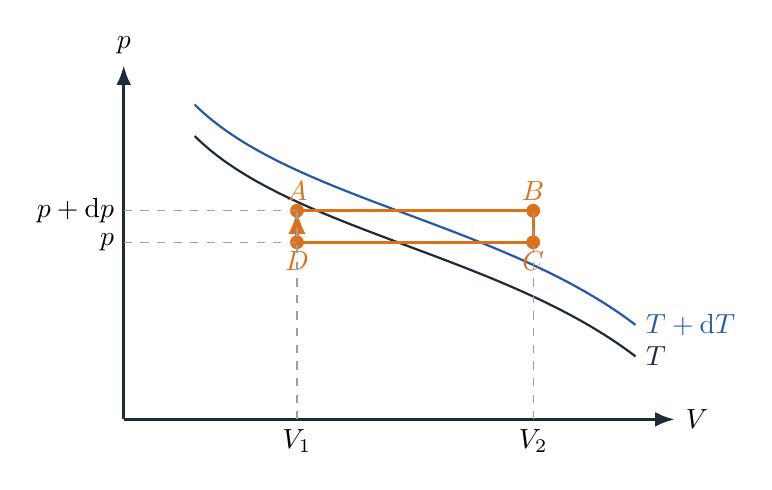
\begin{tikzpicture}[scale=1]
  \draw[axis] (0,0)--(7,0) node[right] {$V$};
  \draw[axis] (0,0)--(0,4.5) node[above] {$p$};
  \draw[blue,thick] (.9,4) .. controls (2.1,2.8) and (4.8,2.5) .. (6.5,1.2) node[right] {$T+\mathrm dT$};
  \draw[ink,thick] (.9,3.6) .. controls (2.1,2.4) and (4.8,2.1) .. (6.5,.8) node[right] {$T$};
  \coordinate (A) at (2.2,2.65);
  \coordinate (B) at (5.2,2.65);
  \coordinate (C) at (5.2,2.25);
  \coordinate (D) at (2.2,2.25);
  \draw[orange,very thick,-{Latex}] (A)--(B)--(C)--(D)--(A);
  \foreach \p/\lab/\pos in {A/A/above,B/B/above,C/C/below,D/D/below}{\fill[orange] (\p) circle(2.5pt) node[\pos] {$\lab$};}
  \draw[guide] (2.2,0) node[below] {$V_1$}--(A);
  \draw[guide] (5.2,0) node[below] {$V_2$}--(B);
  \draw[guide] (0,2.25) node[left] {$p$}--(D);
  \draw[guide] (0,2.65) node[left] {$p+\mathrm dp$}--(A);
\end{tikzpicture}

% 8 solution-04
\begin{tikzpicture}[x=1cm,y=1cm,font=\small]

\node[draw=orange,align=left,text width=7cm] at (0,0) {逐字采用题设 $M=-\mu_0B$：\\[6pt]$\Delta S=-\mu_0B_cB_c'$\\[6pt]形式数值约 $4.08\times10^{-9}$\\[6pt]与题给 SI 磁导率单位不相容；不得标成 $\mathrm{J/K}$};
\node[draw=blue,align=left,text width=7cm] at (8.7,0) {改用 SI 磁化强度 $M=-B/\mu_0$：\\[6pt]$\Delta s=-B_cB_c'/\mu_0$\\[6pt]$\Delta s\simeq2.61\times10^3\ \mathrm{J\,m^{-3}\,K^{-1}}$\\[6pt]总熵变还需要样品体积，原题未给};

\end{tikzpicture}

% 9 question-05
\begin{tikzpicture}[x=1cm,y=1cm,font=\small]

\draw[axis] (-2,0)--(2.2,0) node[right] {$kx$};\draw[axis] (0,-2)--(0,2.2) node[above] {$ky$};
\foreach \x in {-1.2,-.6,.6,1.2}{\foreach \y in {-1.2,-.6,.6,1.2}{\node[blue] at (\x,\y) {$\odot$};}}\draw[body] (.45,.4) circle(.22);\draw[vec] (.67,.4) arc(0:220:.22);\node[right] at (.8,.45) {$I>0$};
\node[align=center] at (0,-2.8) {$B=B_0\cos kx\cos ky$；本图限于 $|kx|,|ky|<\pi/2$\\外部区域还会出现反向磁场，小环电流取逆时针为正};

\end{tikzpicture}

% 10 solution-05
\begin{tikzpicture}[x=1cm,y=1cm,font=\small]

\draw[axis] (-1.6,0)--(1.6,0) node[right] {$kx$};\draw[axis] (0,0)--(0,2.4) node[above] {归一化量};\draw[blue,very thick,domain=-1.5:1.5,samples=100] plot(\x,{cos(\x r)});\draw[orange,very thick,domain=-1.5:1.5,samples=100] plot(\x,{((2-cos(\x r))^2-1)/2});
\node[align=left,anchor=west] at (3,1.3) {取 $y=0,\ LI_0=B_0S$ 作图\\[6pt]蓝：$B/B_0=\cos kx$\\[6pt]橙：$(U-U_0)/(I_0B_0S)$\\[6pt]$U=(\Lambda-SB)^2/(2L)$\\[6pt]原点是小振动平衡点};

\end{tikzpicture}

% 11 question-06
\begin{tikzpicture}[
  x={(.95cm,.32cm)},y={(1cm,0cm)},z={(0cm,1cm)},scale=.78,
  nodept/.style={circle,fill=white,draw=ink,inner sep=1.15pt,line width=.7pt}
]
  % 先画向远处延伸的四条纵棱，再画各个方形截面，突出“方形管”结构。
  \foreach \y/\z in {0/0,2.4/0,0/2.4,2.4/2.4}{
    \draw[body] (0,\y,\z)--(6.65,\y,\z);
    \draw[-{Latex[length=2.1mm]},draw=ink!60,thick]
      (6.45,\y,\z)--(7.25,\y,\z);
  }
  \foreach \n in {0,1.6,3.2,4.8,6.4}{
    \draw[body,draw=ink!78]
      (\n,0,0)--(\n,2.4,0)--(\n,2.4,2.4)--(\n,0,2.4)--cycle;
    \foreach \y/\z in {0/0,2.4/0,0/2.4,2.4/2.4}
      \node[nodept] at (\n,\y,\z) {};
  }
  % 最近的封闭端面加浅色底，避免四条纵棱与端面混淆。
  \fill[blue!6,opacity=.65]
    (0,0,0)--(0,2.4,0)--(0,2.4,2.4)--(0,0,2.4)--cycle;
  \draw[body,line width=1.25pt]
    (0,0,0)--(0,2.4,0)--(0,2.4,2.4)--(0,0,2.4)--cycle;
  \fill[orange] (0,0,2.4) circle(3.2pt) node[left=3pt] {$A$};
  \fill[red] (0,2.4,0) circle(3.2pt) node[right=4pt] {$B$};
  \fill[green] (0,0,0) circle(3.2pt) node[left=4pt] {$C$};
  \node[blue!70!black,fill=white,inner sep=1.5pt] at (0,1.2,3.35) {封闭端面};
  \node[anchor=west,align=left,fill=white,inner sep=2pt]
    at (7.05,2.75,1.55) {向右后方无限延伸\\[-2pt]$n\to\infty$};
  \node[anchor=north,fill=white,inner sep=2pt]
    at (3.25,1.2,-1.35) {所有横向边与纵向边的电阻均为 $r$};
\end{tikzpicture}

% 12 solution-06
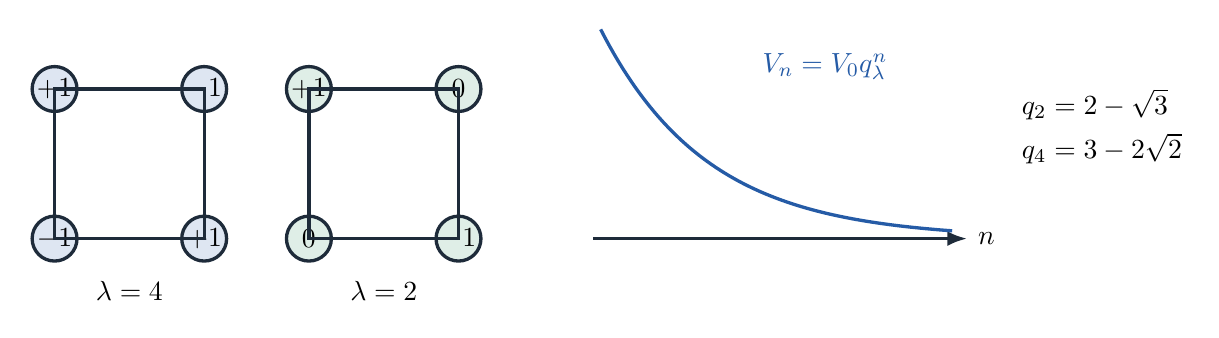
\begin{tikzpicture}[scale=.95]
  \begin{scope}[xshift=-4.2cm]
    \foreach \p/\v in {(0,2)/{+1},(2,2)/{-1},(2,0)/{+1},(0,0)/{-1}}{
      \filldraw[fill=blue!15,body] \p circle(.3) node {$\v$};
    }
    \draw[body] (0,0)--(2,0)--(2,2)--(0,2)--cycle;
    \node at (1,-.7) {$\lambda=4$};
  \end{scope}
  \begin{scope}[xshift=-.8cm]
    \foreach \p/\v in {(0,2)/{+1},(2,2)/{0},(2,0)/{-1},(0,0)/{0}}{
      \filldraw[fill=green!15,body] \p circle(.3) node {$\v$};
    }
    \draw[body] (0,0)--(2,0)--(2,2)--(0,2)--cycle;
    \node at (1,-.7) {$\lambda=2$};
  \end{scope}
  \draw[axis] (3,0)--(8,0) node[right] {$n$};
  \draw[blue,very thick,domain=3.1:7.8,samples=80]
    plot(\x,{3*exp(-.7*(\x-3))});
  \node[blue] at (6.1,2.3) {$V_n=V_0q_\lambda^n$};
  \node[align=left,anchor=west] at (8.6,1.5)
    {$q_2=2-\sqrt3$\\[4pt]
     $q_4=3-2\sqrt2$};
\end{tikzpicture}

% 13 question-07
\begin{tikzpicture}[x=1cm,y=1cm,font=\small]

\draw[axis] (-2.5,0)--(2.5,0) node[right] {$x$};\draw[axis] (0,0)--(0,3) node[above] {$V(x)$};\draw[blue,very thick,domain=-2:2,samples=100] plot(\x,{.5*\x*\x});\draw[orange,thick] (-1.4142,1)--(1.4142,1) node[right] {$E-mc^2$};\draw[guide] (-1.4142,0)--(-1.4142,1);\draw[guide] (1.4142,0)--(1.4142,1);\node[below] at (-1.4142,0) {$-b$};\node[below] at (1.4142,0) {$b$};\node at (0,3.7) {转折点满足 $V(b)=E-mc^2$};

\end{tikzpicture}

% 14 solution-07
\begin{tikzpicture}[x=1cm,y=1cm,font=\small]

\draw[axis] (0,0)--(3.4,0) node[right] {$\eta=kb^2/(2mc^2)$};\draw[axis] (0,0)--(0,1.4) node[above] {$v_{\max}/c$};\draw[blue,very thick,domain=0:3,samples=150] plot(\x,{sqrt(1-(1+\x)^(-2))});\draw[guide] (0,1)--(3,1);\node[left] at (0,1) {$1$};\node[align=left,anchor=west] at (6.8,1.5) {$v_{\max}/c=\sqrt{1-(1+\eta)^{-2}}$\\[6pt]$T=2\pi\sqrt{m/k}\,[1+3\eta/8+O(\eta^2)]$\\[6pt]一阶周期公式只用于 $\eta\ll1$};

\end{tikzpicture}

% 15 question-08
\begin{tikzpicture}[scale=1]
  \fill[blue!8] (-4,0) rectangle (4,2.8);
  \fill[green!8] (-4,-2.3) rectangle (4,0);
  \draw[body] (-4,0)--(4,0) node[right] {界面 $x$};
  \draw[guide] (0,-2.1)--(0,2.6) node[above] {法线};
  \draw[vec] (-3,2.4)--(0,0);
  \draw[vec] (-2.5,2.4)--(.35,0);
  \draw[force] (0,0)--(3,2.4);
  \draw[force] (.35,0)--(3.35,2.4);
  \draw[blue] (0,1.2) arc[start angle=90,end angle=141,radius=1.2];
  \node[blue] at (-.8,1.2) {$\theta$};
  \node at (-3.3,1.9) {入射角谱};
  \node[red] at (3.1,1.9) {反射角谱};
  \node[green] at (3,-1.5) {倏逝场};
\end{tikzpicture}

% 16 solution-08
\begin{tikzpicture}[x=1cm,y=1cm,font=\small]

\draw[axis] (-2.5,0)--(4.5,0) node[right] {$x$};\draw[blue,very thick,domain=-2.3:2.3,samples=120] plot(\x,{1.5*exp(-\x*\x)});\draw[orange,very thick,domain=-1.3:3.7,samples=120] plot(\x,{1.5*exp(-(\x-1)^2)});\draw[guide] (0,0)--(0,1.5);\draw[guide] (1,0)--(1,1.5);\draw[dim] (0,1.9)--(1,1.9) node[midway,above] {$\Delta>0$};
\node[align=left,anchor=west] at (5.3,.9) {$r=e^{i\delta}$，场约定 $e^{i(\omega t-\bm k\cdot\bm r)}$\\[6pt]反射实场：$\cos(k_xx-\omega t-\delta)$\\[6pt]$\Delta=\delta'(\theta)/(k\cos\theta)$\\[6pt]蓝：几何反射峰；橙：带相位的波包峰};

\end{tikzpicture}
\end{document}
